\documentclass[11pt, a4paper, twoside]{report}
\usepackage{graphicx}
\usepackage{url}
\usepackage{amsmath}
\usepackage[margin=0.85in]{geometry}
\usepackage{listings}
\usepackage{minted}
\usemintedstyle{vs}
\usepackage{float}
\usepackage{fancyhdr}
\usepackage{indentfirst}
\usepackage[inline]{enumitem}
\usepackage{tabularx}
\usepackage[dvipsnames]{xcolor}
\usepackage[belowskip=0pt,aboveskip=0pt,font=small,labelfont=small]{caption}
\captionsetup{width=\linewidth}

\def \courseNumber {EE2703}
\def \assignmentNumber {Final Exam}
\def \myName {Akilesh Kannan}
\def \rollNumber {EE18B122}

\setlength\intextsep{0pt}
\graphicspath{{Plots/}}
\setlist[itemize]{noitemsep, topsep=0pt}
\fancyhead[RO,LE]{\courseNumber : \assignmentNumber}
\fancyhead[LO,RE]{\myName\ (\rollNumber)}
\cfoot{\thepage}

\title{\Huge{\textbf{\courseNumber : \assignmentNumber}}}
\author{\Large{\myName\ (\rollNumber)}}
\date{July 31, 2020}

\pagestyle{fancy}

\renewcommand\thesection{\arabic{section}}

\begin{document}
\maketitle
    \section{Problem Description}
        The Laplace equation \eqref{Eq1} is a special case of Poisson’s equation applicable in a region where the charge concentration is zero inside. It provides for a simple condition for the electric potential function $\phi$, thus making it mathematically easy to compute the potential distribution in the region. This method is widely used to perform numerical simulations of regions with given boundary conditions.
        \begin{equation}
            \nabla^2\phi = 0
            \label{Eq1}
        \end{equation}

        In 2 dimensions, Equation \eqref{Eq1} reduces to the PDE,

        \begin{equation}
            \frac{\partial^2 \phi}{\partial x^2} + \frac{\partial^2 \phi}{\partial y^2} = 0
        \end{equation}

        For numerical simulation, it can be proved that \cite{Assgn5} the potential at any point (i, j) can be written as
            \begin{equation}
                \phi_{i, j} = \frac{\phi_{i+1, j}+\phi_{i-1, j}+\phi_{i, j+1}+\phi_{i, j-1}}{4}
                \label{Eq3}
            \end{equation}

        Equation \eqref{Eq3} is valid for those points which aren't at the interface between 2 dielectrics. For those points, the potentials can be written as
            \begin{equation}
                \phi_{interface} = \frac{\epsilon_{ra}\phi_a + \epsilon_{rb}\phi_b}{\epsilon_{ra}+\epsilon_{rb}}
                \label{Eq4}
            \end{equation}
        where the subscript $a$ denotes above the boundary and $b$, for below the boundary.\\

        The main objective of the problem given is to analyse the dependence of a metal tank's capacitance on the height of fluid (a dielectric) in the tank, and how it affects the resonant frequency of an external RLC circuit, using the tank as it's capacitor. The tank's side and bottom walls are kept grounded, while the top is connected to the RLC circuit, and is assumed to be at 1V.\\

        The angular resonant frequency of the RLC circuit is given by
            \begin{equation}
                \omega_o = \frac{1}{\sqrt{LC}}
                \label{Eq5}
            \end{equation}

        It is required to solve Laplace's equation inside the tank (shown in \ref{fig:tank}) to find the potential distribution inside it, and from it, the capacitance seen by the circuit and the resonant frequency of the circuit.

        \begin{figure}[H]
            \centering
            \includegraphics[scale=0.3]{Screenshot 2020-08-01 at 10.53.58 AM.png}
            \caption{The tank}
            \label{fig:tank}
        \end{figure}

        \subsection{Notations and Conventions followed in program}
        \begin{enumerate}
            \item After meshing the potential in the region into a M × N mesh of nodes, the boundary electric potential is assigned such that the top row of nodes is completely assigned to be 1V on the top plate, while the rest of the boundary is assigned to be having 0V (GND).
            \item The origin is taken to be the bottom-left corner of the tank.
        \end{enumerate}
    \section{Formulating a method to estimate the height of the tank}
        Given the resonant angular frequency $\omega_o$ and the value of $L$, the capacitance of the tank is
            \begin{equation}
                C = \frac{1}{L\omega_o^2}
            \end{equation}
        Now that we know the capacitance of the tank, we need a relation between the height of the fluid in the tank and it's capacitance.\\

        If the charge on the top plate (at 1V) is given by $Q_{top}$, then the capacitance is simply
            \begin{equation}
                C = \frac{Q}{V} = \frac{Q_{top}}{1V} = Q_{top}
                \label{Eq7}
            \end{equation}

        Therefore, we need to find the total charge accumulated on the top surface of the tank.\\

        Using Laplace's Equation \eqref{Eq3} iteratively, we can find the potential at any point inside the tank. Using these values, we can find the Electric field ($\vec{E}$ by taking the negative gradient of the potential.
            \begin{equation}
                \vec{E} = \nabla \phi
                \label{Eq8}
            \end{equation}

        We find the electirc field at the center of a square enclosed by 4 mesh nodes [$(m, n),\, (m+1, n),\, (m, n+1)$ and $(m+1, n+1)$] as shown below. Here, $\delta$ is the separation between 2 adjacent nodes.
            \begin{gather}
                E_{x,(m+0.5, n+0.5)} = -\frac{1}{2}\left(\frac{\phi_{m, n+1}-\phi_{m,n}}{\delta} + \frac{\phi_{m+1, n+1}-\phi_{m+1,n}}{\delta} \right)\\
                E_{y,(m+0.5, n+0.5)} = -\frac{1}{2}\left(\frac{\phi_{m+1, n}-\phi_{m,n}}{\delta} + \frac{\phi_{m+1, n+1}-\phi_{m+1,n+1}}{\delta} \right)
            \end{gather}

        At the boundaries (i.e., the walls of the tank), the $\vec{E}$ is normal to it, as the walls are ideal conductors, and they are related to the surface charge density as,
            \begin{equation}
                \vec{E} = \frac{\sigma}{\epsilon_o\epsilon_r}\hat{n}
                \label{Eq11}
            \end{equation}
        where, $\hat{n}$ is the unit vector in the normal direction to the surface.\\

        Now, we have a simple relation between the charge on the surface and the electric field \textit{normal} to it. Summing the charges at each point on the surface should give us the total charge $Q$ on the surface. The calculation of capacitance of the tank can now be easily done with \eqref{Eq7} and $Q_{top}$, which is obtained from \eqref{Eq8}-\eqref{Eq11}.\\

        Doing the above procedure for different heights of the fluid will give us a relationship between $h$, the height of the fluid, and $C$, the capacitance offered by the tank. We can then fit a curve to the $h-C$ values obtained to calculate $h$ from $C$.

    \section{Solving Laplace's Equation in the Tank}
        As mentioned before, to solve Laplace's equation \eqref{Eq1} numerically, we can iteratively calculate the potential at each point as the average of it's neighbours. We stop the iterative calculation when we have reached a specified accuracy, in the error between successive iterations. The following code implements the iterative calculator.

        \inputminted[linenos, breaklines=True, fontsize=\footnotesize]{python}{laplaceSolver.py}

        A contour plot of the potential distribution (for $h = 0.5L_y$) is shown below.

        \begin{figure}[H]
            \centering
            \setlength\tabcolsep{2pt}
            \begin{tabular}{c c}
                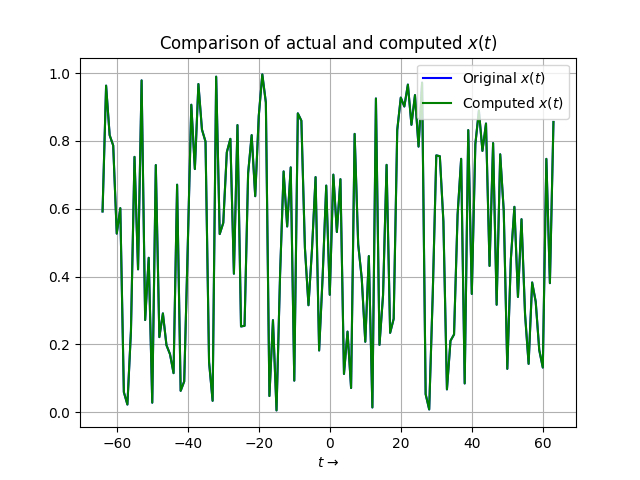
\includegraphics[scale=0.5]{Fig0.png} &
                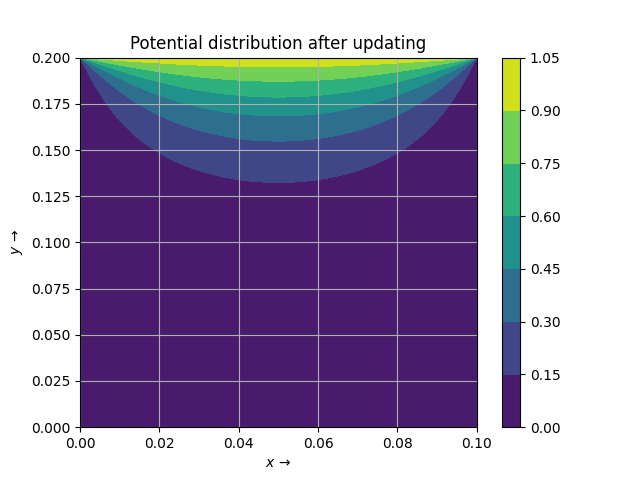
\includegraphics[scale=0.5]{Fig1.png}\\
            \end{tabular}
            \caption{Potential Distribution - \textit{left}: initialisation, \textit{right}: iteratively calculated}
        \end{figure}

        \subsection{Parallelising the computation}
            Computing potential values for a 200x100 grid iteratively is an awfully slow process due to heavy computational complexity and the general slowness of the Python language due to it's interpreted nature. This can be parallelised to make the updation faster. \texttt{Numpy} arrays are internally implemented in C, with a wrapper function to use it in Python.

            Numpy arrays can also be "\textit{vectorized}", i.e., optimized, pre-compiled code written in a low-level language (e.g. C) to perform mathematical operations over a sequence of data, due to the fact that they are homogeneous data types.

            Thus, executing the operations in C helps optimize the code, as each row of the array is operated on in parallel.

            One thing to keep in mind is that the row corresponding to the interface has to be done separately. For that, we first create a copy of the current potential array. Then update the potentials of each row in the array by averaging the potentials of it's neighbours, including the interface row, update the interface row using Equation (4), with the values from the copied array, and then apply boundary conditions.

            This has been done in lines \texttt{49} - \texttt{59} in the above code.

        \subsection{Error Estimation and Fitting}
            The accuracy for the solution is passed as the argument \texttt{accuracy} to the function \texttt{solve()}, and the maximum number of iterations to be performed, \texttt{No} is also passed to it.

            At each iteration, the maximum error between the updated values and the values got in the previous iteration are compared, and if the difference is less than \texttt{accuracy}, then the solver stops iterating anymore. If not, it keeps continuing till it reaches \texttt{No}.\\

            This method of iteratively solving Laplace's equation leads to an exponential relation between the errors and iterations (after a certain number of iterations) \cite{Assgn5}. We can thus fit the error-iteration curve to an exponential of the form $y = Ae^{Bx}$.

            Figure (3) shows the actual error and the error fitted using least-squares method.

            \begin{figure}[H]
                \centering
                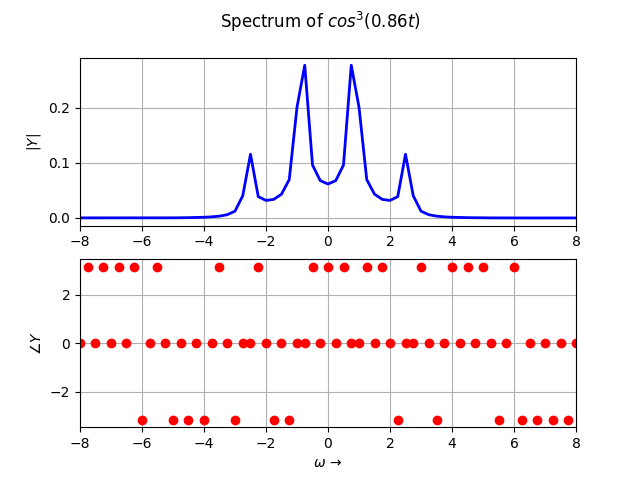
\includegraphics[scale=0.75]{Fig2.png}
                \caption{Exponential Fit of error with iteration}
            \end{figure}

    \section{Calculation of $\vec{E}$ from potential distribution}
        As described in Equations \eqref{Eq8} - \eqref{Eq11}, we can find the electric field at the center of the mesh cells by averaging the gradients of the potential on it's sides. The following code snippet accomplishes the same

        \inputminted[linenos, breaklines=True, fontsize=\footnotesize]{python}{findEField.py}

        \textbf{Disclaimer:} The plots presented in this section have been generated for a $h/L_y$ ratio of 0.5, as asked in the Question Paper.

        \subsection{The normal $\vec{D}$ continuity}
            The boundary conditions at the interface between air and fluid require the normal component of $\vec{D}$ to be continuous across it:
            \begin{gather}
                D_{na} = D_{nb}\\
                \epsilon_a E_{na} = \epsilon_b E_{nb}
            \end{gather}

            Figure 4 shows the plot of $\vec{D_n}$ above and below the interface. We can clearly see that the two are indeed equal.

            \begin{figure}[H]
                \centering
                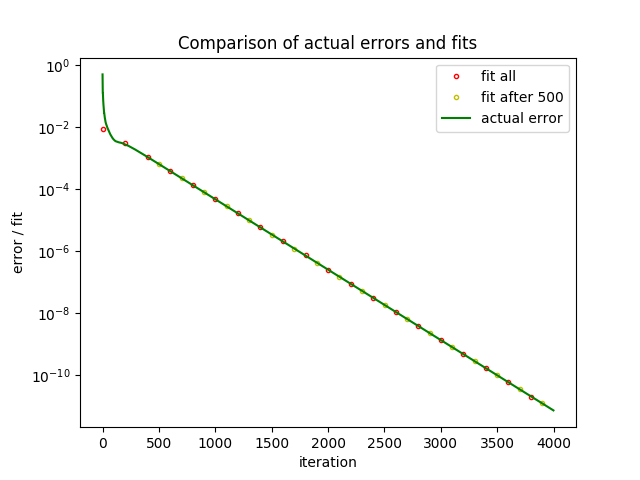
\includegraphics[scale=0.75]{Fig4.png}
                \caption{Continuity of $\vec{D_n}$ across interface}
                \label{fig:Fig4}
            \end{figure}

        \subsection{The tangential $\vec{E}$ continuity}
            The boundary conditions at the interface between air and fluid require the tangential component of $\vec{E}$ to be continuous across it:
            \begin{equation}
                E_{ta} = E_{tb}
            \end{equation}

            Figure 5 shows the plot of $\vec{E_t}$ above and below the interface. We can clearly see that the two are indeed equal.

            \begin{figure}[H]
                \centering
                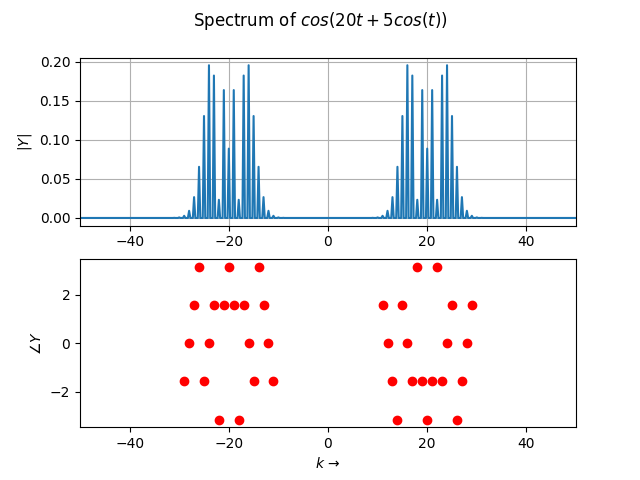
\includegraphics[scale=0.75]{Fig5.png}
                \caption{Continuity of $\vec{E_t}$ across interface}
                \label{fig:Fig4}
            \end{figure}

        \subsection{Direction of $\vec{E}$ at interface}
            Let us take $\theta_a$ and $\theta_b$ as the angles made by $\vec{E}$ with the y-axis (normal to interface), above and below the interface respectively.

            From boundary conditions imposed by Maxwell's Equations, we get,
                \begin{gather}
                    E_a^{||} = E_b^{||}\\
                    \epsilon_a E_a^{\perp} = \epsilon_b E_b^{\perp}
                \end{gather}
            or, in another form,
                \begin{align}
                    \frac{E_a^{||}}{\epsilon_a E_a^{\perp}} = \frac{E_b^{||}}{\epsilon_b E_b^{\perp}}\\
                    \implies \frac{tan\,\theta_a}{\epsilon_a} = \frac{tan\,\theta_b}{\epsilon_b}\\
                    \implies \frac{tan\,\theta_a}{tan\,\theta_b} = \frac{\epsilon_a}{\epsilon_b}
                \end{align}
            i.e., the ratio of the tangents of the angles is a constant.\\

            Thus, Snell's Law, which states that \textit{"the ratio of the sines of the angles of incidence and refraction of a wave are constant when it passes between two given media"}\cite{SNELL}, will not be valid.\\

            This is expected because, Snell's law holds good only for \textit{Electromagnetic Waves}, as given in the above statement, and not for \textit{Electrostatic} distributions.

            Given below are plots that confirm these inferences.
            \begin{figure}[H]
                \centering
                \setlength\tabcolsep{2pt}
                \begin{tabular}{cc}
                    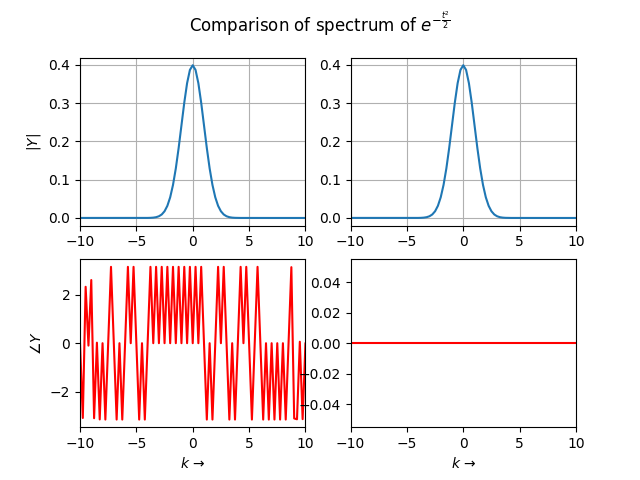
\includegraphics[scale=0.5]{Fig6.png} &
                    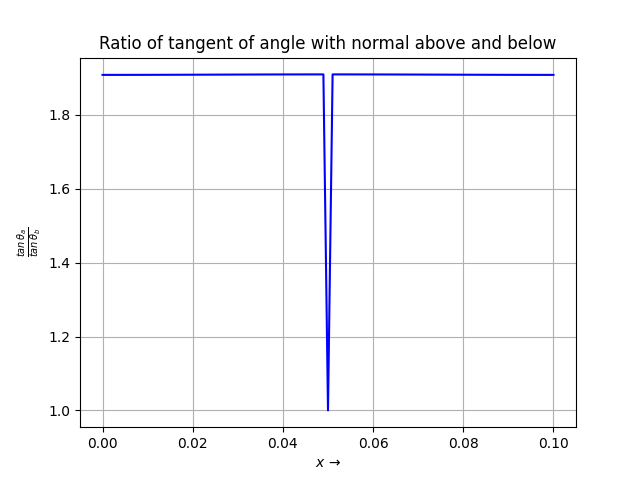
\includegraphics[scale=0.5]{Fig7.png}\\
                \end{tabular}
                \caption{Charge variation with $h$ - \textit{left}: $Q_{top}$, \textit{right}: $Q_{fluid}$}
            \end{figure}

    \section{Dependence of $Q_{top}$ on fluid height $h$}
        With the above calculated $\vec{E}$, we can find the total charge on the top plate $Q_{top}$ for different values of $h$, going from $h=0.1L_y$ to $h=0.9L_y$, as described by Equation \eqref{Eq11}.

        Similarly we can calculate $Q_{fluid}$ by summing up the charges on the bottom plate, and on the side-plates, only along the regions submerged in the fluid.
            \begin{equation}
                Q_{fluid} = Q_{bottom} + Q_{left, sub} + Q_{right, sub}
            \end{equation}\\

        We get the following plots, that describe the relation between $Q_{top}$ vs. $h/L_y$  and $Q_{fluid}$ vs. $h/L_y$.

        \begin{figure}[H]
            \centering
            \setlength\tabcolsep{2pt}
            \begin{tabular}{cc}
                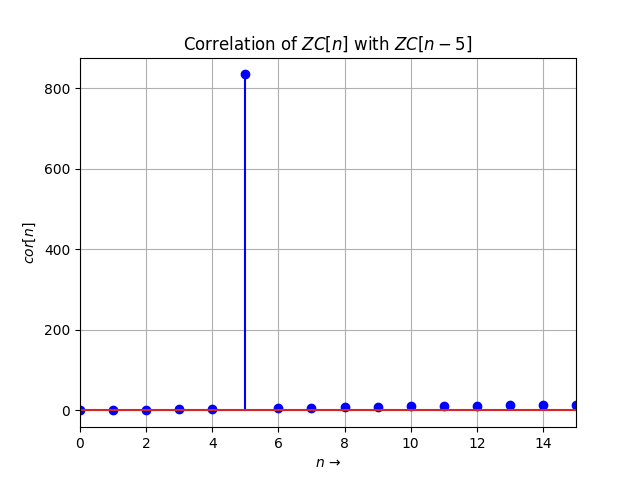
\includegraphics[scale=0.5]{Fig8.png} &
                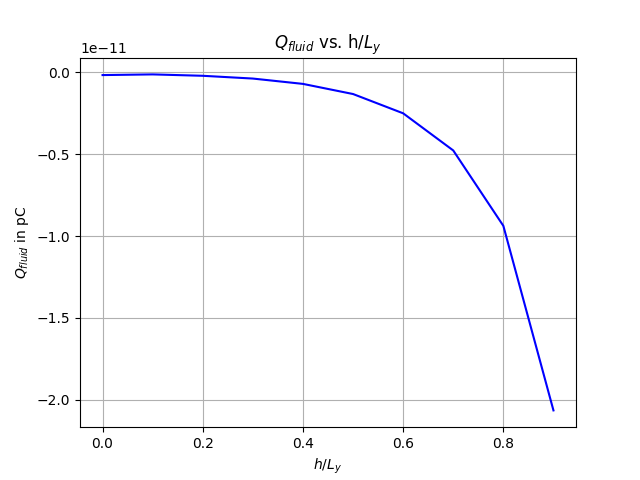
\includegraphics[scale=0.5]{Fig9.png}\\
            \end{tabular}
            \caption{Charge variation with $h$ - \textit{left}: $Q_{top}$, \textit{right}: $Q_{fluid}$}
        \end{figure}

        Qualitatively, as the height of the dielectric increases, the capacitance must increase as, the tank can store more charge in the dielectric compared to air. This is indeed observed. in the plot. But, the plots also describe that the rate of increase isn't linear, but looks like an exponential.

        One can do the following thought experiment to understand why the increase isn't expected to be linear.
        Consider an increase of $0.1L_y$ in the height of the fluid. This means that the height of the air column inside decreases by $0.1L_y$. The strength of the electric field vector $\vec{E}$, is much more stronger near the top plate due to the large drop of 1V in a small region. So, naturally we expect that the change in the charge on the surface will be more for the same $0.1L_y$ change in the height of the fluid, if that change takes place near the top. So, \textbf{we don't expect the variation of the charge on the top surface $Q_{top}$ to be linearly varying with $h$}.

    \section{Estimation of height using resonant frequency}
        Now that we have got an approximate relationship between $h$ and $Q_{top}$ (= $C$), we can now find the height $h$, given the capacitance $C$, which is calculated using Equation \eqref{Eq5}.

        We can use two methods to find $h$ from $C$:
        \begin{enumerate}
            \item We can use a simple linear interpolation to find an approximate analytical relation, that is piece-wise linear, between $h$ and $C$, which we can then use to find $h$, given $C$.
            \item From the plot of $Q_{top}$ vs. $h$, we can see that it looks approximately of the form of $Q_{top} = \frac{1}{ah+b}$, which is expected because the tank can be approximately modelled as a series combination of an air capacitor of width $L_y-h$ and another fluid-filled capacitor of width $h$ - which results in a net capacitance of $\frac{\epsilon_o \epsilon_r A}{h(1-\epsilon_r)+\epsilon_rL_y}$, where $A$ is the area of cross-section. Thus, we can try to fit a rectangular hyperbola $y = \frac{1}{ax+b}$ to the observed plot, and get a relation between $C$ and $h$.
        \end{enumerate}

    \section{Conclusion}
        A numerical solution to an analytically complex problem of finding the potential distribution inside the tank has been obtained, to a high degree of accuracy. Though it is not exact, this serves to help us analyse how the charge distribution and in turn, potential distribution changes with the height of the fluid, without using complex math and more importantly, efficiently.


    \bibliography{references}
    \bibliographystyle{abbrv}
\end{document}
